\documentclass{beamer}[10]
\usepackage{pgf}
\usepackage{beamerthemesplit}
\usepackage{array}
\usepackage{wrapfig}
\usepackage{varwidth}
%\usepackage{enumitem}
\usepackage{listings}
\lstset{language=bash,
	basicstyle=\ttfamily\scriptsize,		
	keywordstyle=\color{blue}\ttfamily,
	morekeywords={peter@kbpet},
	alsoletter={:~$},
	morekeywords=[2]{peter@kbpet:},
	keywordstyle=[2]{\color{red}},
	literate={\$}{{\textcolor{red}{\$}}}1 
	{:}{{\textcolor{red}{:}}}1
	{~}{{\textcolor{red}{\textasciitilde}}}1,
	breaklines=true,
	numbers=none,
	numbersep=5pt,
	stepnumber=1
}
\usepackage{algorithm,algpseudocode}
\usepackage{hyperref}
\usepackage{pdfpc-commands}
\usepackage{pgfpages}

%\usepackage{natbib}
\bibliographystyle{apalike}

\definecolor{kugreen}{RGB}{50,93,61}
\definecolor{kugreenlys}{RGB}{132,158,139}
\definecolor{kugreenlyslys}{RGB}{173,190,177}
\definecolor{kugreenlyslyslys}{RGB}{214,223,216}
\definecolor{kublue}{RGB}{0,101,163}
\definecolor{kubluelys}{RGB}{132,158,139}
\definecolor{kubluelyslys}{RGB}{173,190,177}
\definecolor{kubluelyslyslys}{RGB}{214,223,216}
\setbeamercovered{transparent}
\mode<presentation>
\usetheme[numbers,totalnumber,compress,sidebarshades]{PaloAlto}
%\setbeamertemplate{footline}[frame number]

\usecolortheme[named=kublue]{structure}
\useinnertheme{circles}
\usefonttheme[onlymath]{serif}
\setbeamercovered{transparent}
\setbeamertemplate{blocks}[rounded][shadow=true]
\setbeameroption{show notes on second screen}

\logo{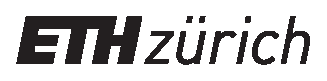
\includegraphics[width=1.5cm]{gfx/eth_logo_kurz_pos}}
\title{Semester Project}
\subtitle{Robust object tracking in 3D by fusing ultra-wideband and vision}
\author{Andreas Ziegler}
\institute{AIT \\ ETH Zürich}
\date{13th of July 2016}

\newcommand{\setlistspacing}[2]{\def\@ld{#1}\expandafter\def\csname
	@list\romannumeral\@ld \endcsname{\leftmargin\csname
		leftmargin\romannumeral\@ld \endcsname
		\topsep    #2
		\parsep    0\p@   \@plus\p@
		\itemsep   #2}}
\makeatother

\begin{document}

\frame { \frametitle{Semester Project}
	\begin{center}
	\LARGE Semester Project \\
	- \\
	Robust object tracking in 3D by fusing ultra-wideband and vision\\
	- \\
	\includegraphics*[height=0.6cm]{gfx/eth_logo_kurz_pos.eps} \hfill
	\includegraphics*[height=0.6cm]{gfx/logo-ait} \hfill
	\includegraphics*[height=0.6cm]{gfx/biwi_logo}
	\end{center}
}

\frame { \frametitle{Contents}
	\tableofcontents
}

\frame{ \frametitle{Motivation}
	\section{Motivation}
	%\subsection{Initial situation}
	\begin{itemize}
	\item Object tracking is an important building block
	\item Most state-of-the-art robust approaches work with predefined objects $\rightarrow$ not engough flexible
	\item Online visual tracking $\rightarrow$ limited labeled data
	\item New approach: Fusion of Ultra-wideband (UWB) and a visual tracker with an Extended Kalman Filter (EKF)
	%\item Using a Kernelized correlation filter
	\end{itemize}
}
\note[enumerate]
{
	\item for many interactive	systems, especially for robotic systems interacting with humans.
	\item 
	\item any such tracking approach has to balance plasticity versus drift, in particular when an object should be re-detected after loss of tracking.
}

\frame{	\frametitle{Related work - Ultra-wideband (UWB)}
	\section{Related work}
	\subsection{UWB}
	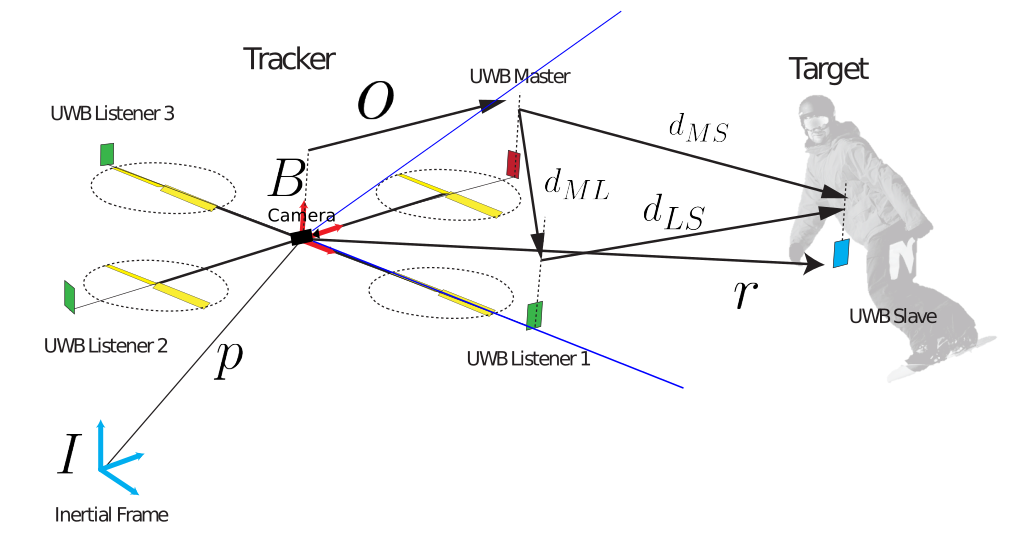
\includegraphics[height=3.5cm]{gfx/system}
	\begin{itemize}
	\item Provides 3D position and velocity information
	\item Accuracy of $\approx 10\textit{cm}$
	\end{itemize}
	\cite{Naegeli:2016}
}

\frame{	\frametitle{Related work - Kernelized correlation filters (KCF)}
	\subsection{KCF}
	\begin{center}
	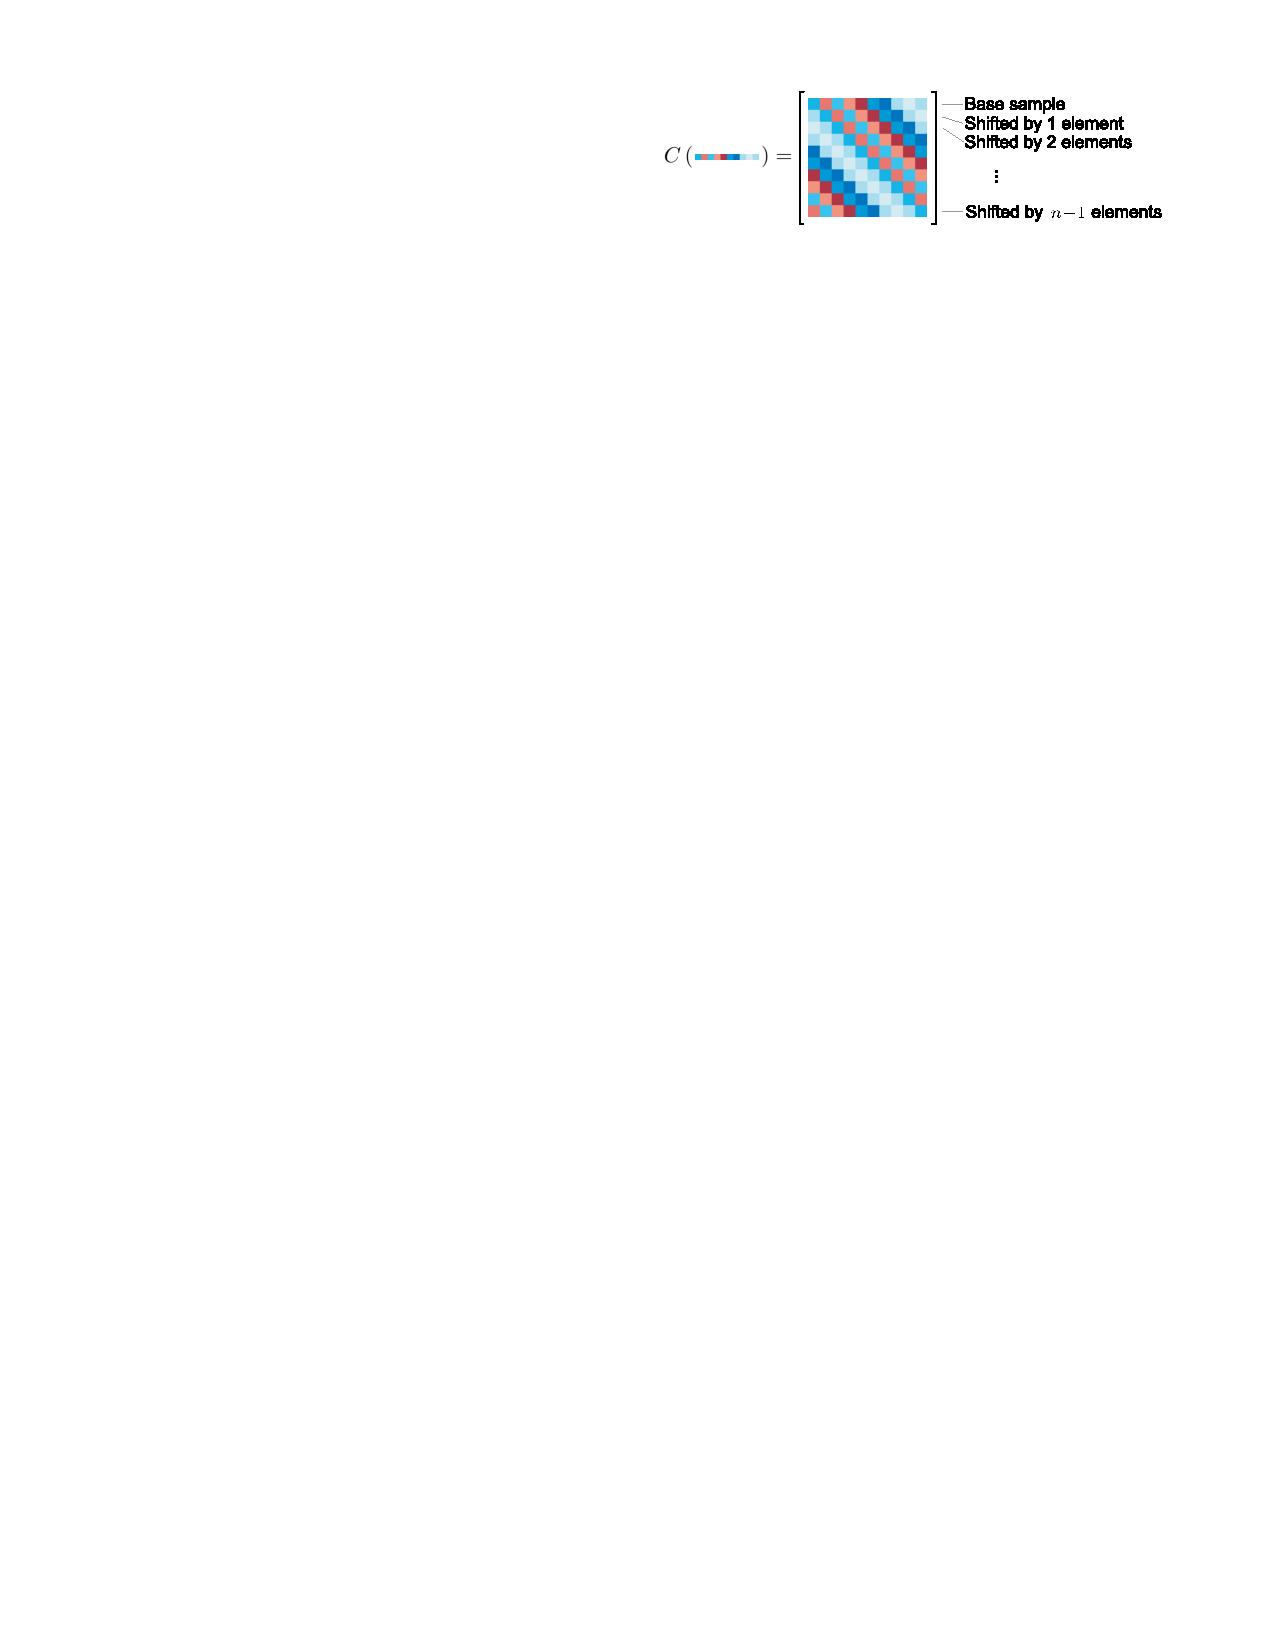
\includegraphics[width=0.5\linewidth]{gfx/circular-1}
	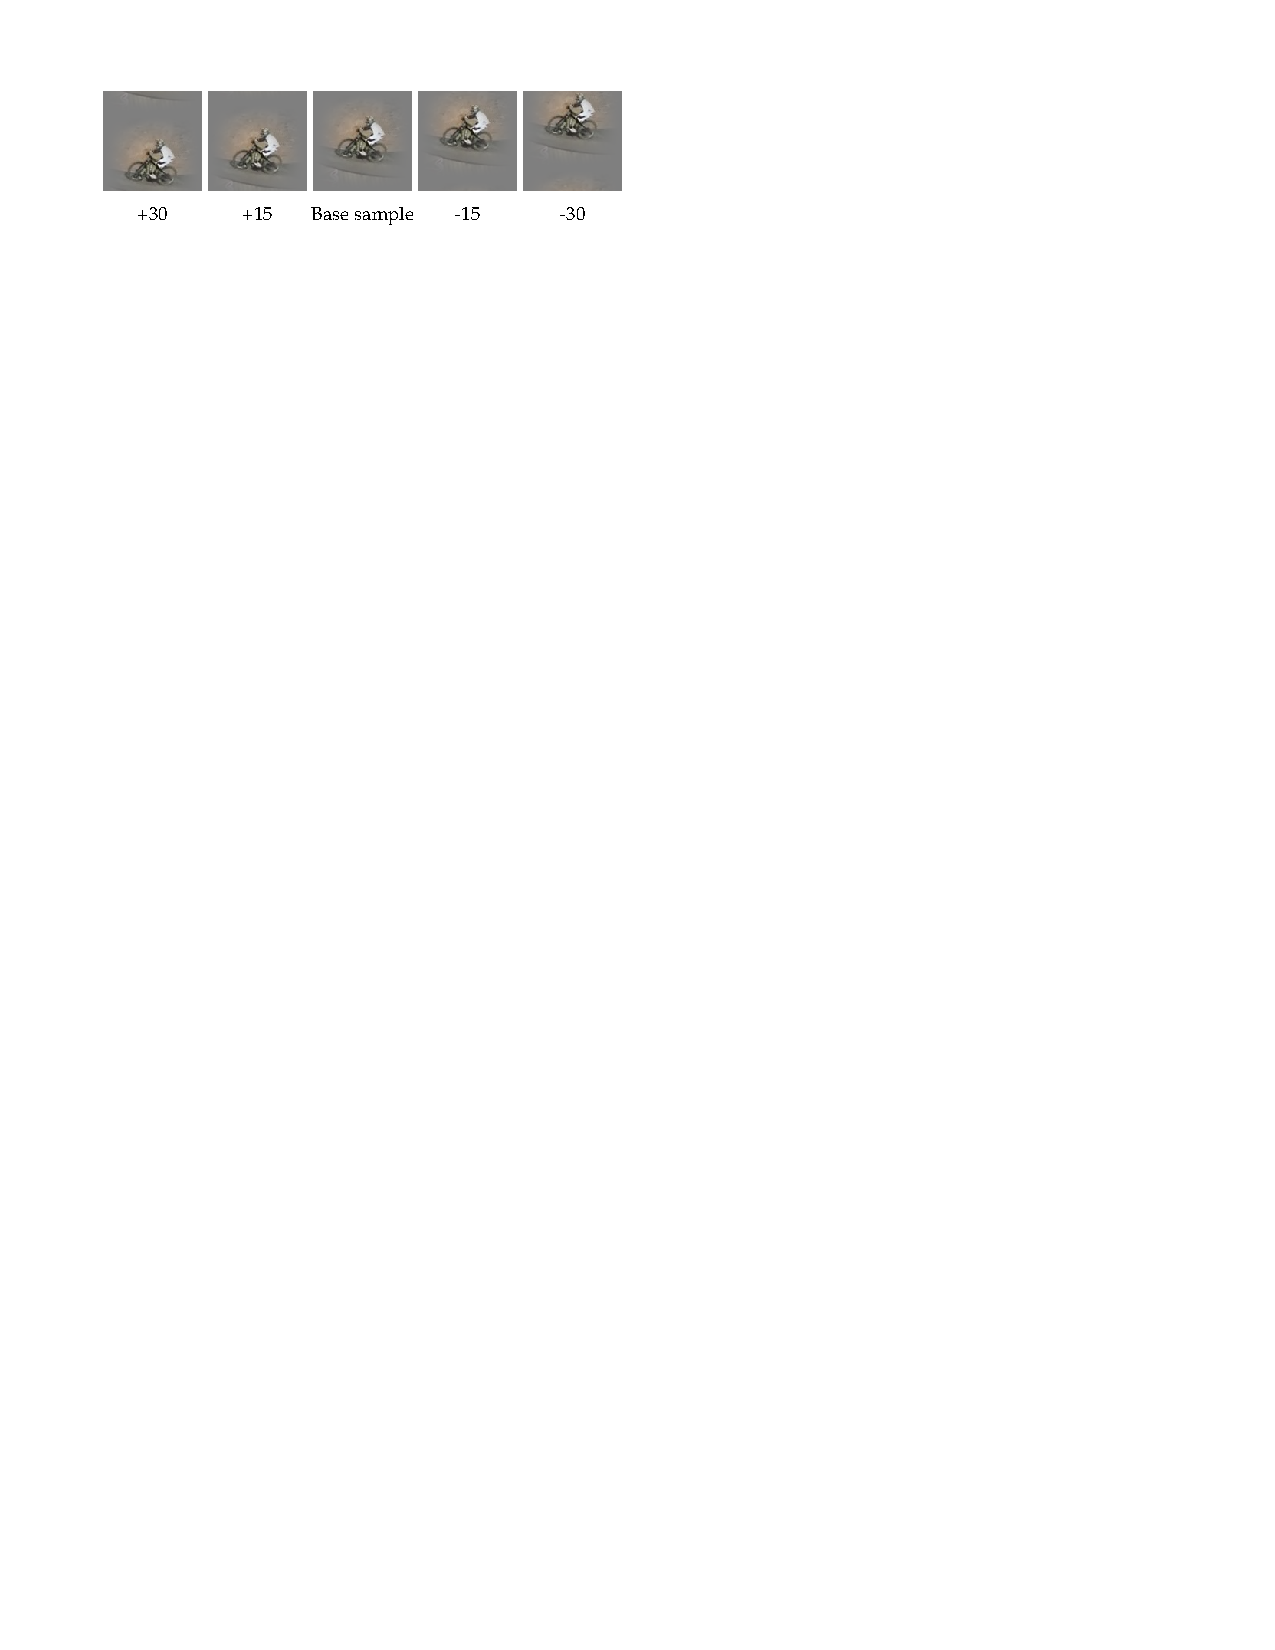
\includegraphics[width=0.5\linewidth]{gfx/circular-2}\let\thefootnote\relax\footnote{Figures from Henriques et al. 2015. High-speed tracking with kernelized correlation filters}
	\end{center}
	\begin{itemize}
	\small
	\item Translated and scaled patches are riddled with redundancies $\rightarrow$ Can be represented as a circulant matrix
	\item Circulant matrices can then be diagonalized with the Discrete Fourier Transform $\rightarrow$ Reduces storage as well as computation
	\item The KCF tracker can be implemented with
	only a few lines of code.
	%\item 3 functions: "train", "detect" and "kernel\_correlation"
	\end{itemize}
	\cite{henriques2015tracking}
}

\frame{	\frametitle{Setup - Mounting}
	\section{Setup}
	\subsection{Mounting}
	\begin{itemize}
	\item Camera calibration
	\item UWB and camera mounting
	\begin{center}
	\includegraphics[height=3.0cm]{gfx/Monitor_cut}
	\end{center}
	\end{itemize}
}

\frame{	\frametitle{Setup - Matching the two coordinate systems}
	\subsection{Matching}
	\begin{center}
	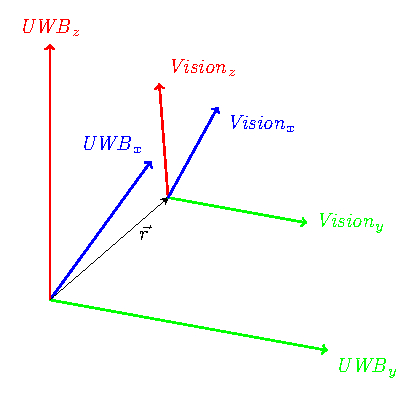
\includegraphics[height=3.0cm]{gfx/coordination_system}
	\end{center}
	\begin{itemize}
	\item ArUco \cite{Aruco2014}:
	\begin{center}
	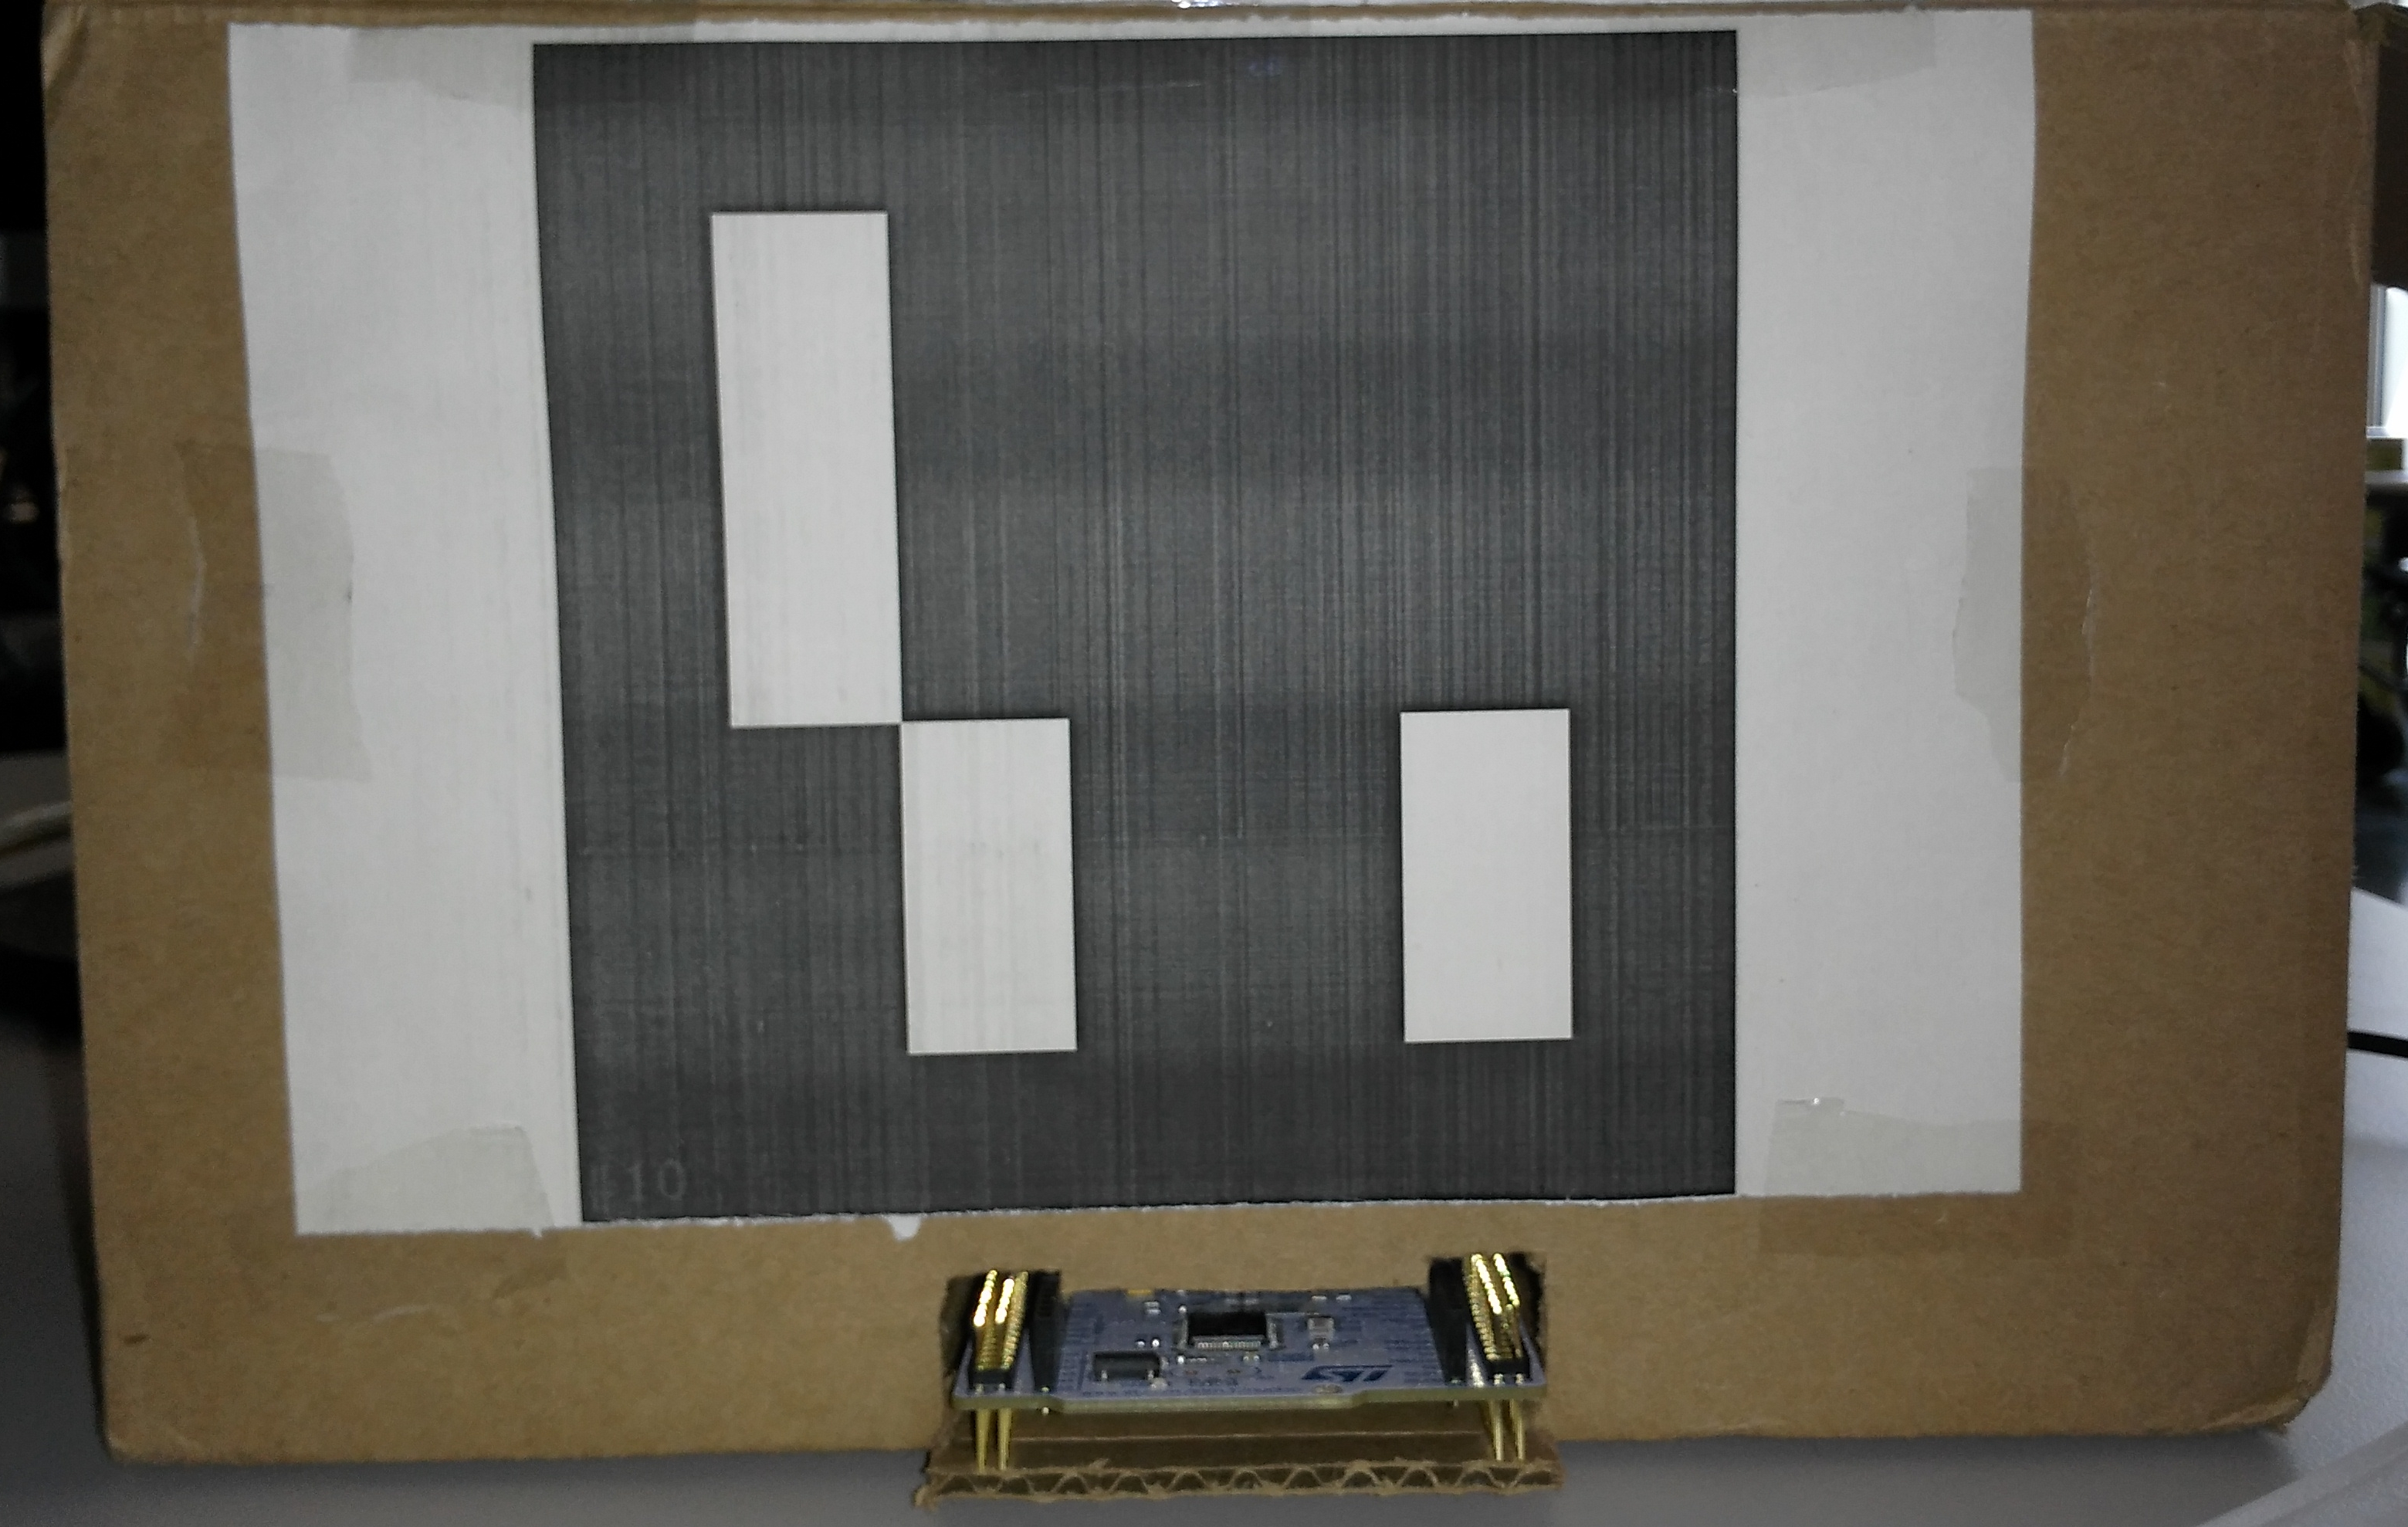
\includegraphics[height=2.0cm]{gfx/Box_cut}
	\end{center}
	\item Kabsch:
	Get rotation matrix $\textbf{U}$ and translation vector $\vec r$ which results in the $\textit{lrms}$
	\end{itemize}
}

\frame{	\frametitle{Setup - Transform between the coordinate systems}
	\subsection{Transform}
	%Transform between the two coordinate systems
	%\begin{center}
	%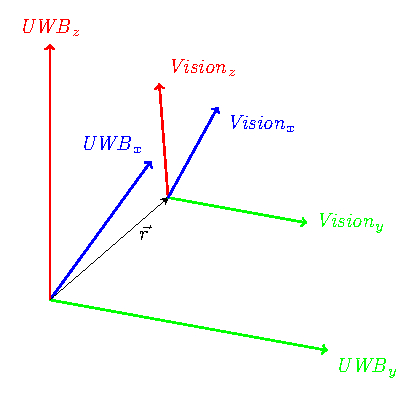
\includegraphics[height=1.5cm]{gfx/coordination_system}
	%\end{center}
	Transform a point:
	\begin{equation}\label{eq:transformation}
	\begin{bmatrix}
	x_{\textit{Vision}} \\
	y_{\textit{Vision}} \\
	z_{\textit{Vision}}
	\end{bmatrix} = \frac{1}{\mathit{scale}} \cdot \textbf{U}
	\Bigg( \begin{bmatrix}
	x_{\textit{UWB}} \\
	y_{\textit{UWB}} \\
	z_{\textit{UWB}}
	\end{bmatrix} - \vec r \Bigg)
	\end{equation}
	Transform the covariance matrix:
	\begin{equation}
	\textbf{C}' = \frac{1}{\mathit{scale}^2} \textbf{U}' \textbf{C} \textbf{U}'^T
	\end{equation}
	where
	\begin{equation}
	\textbf{U}' =
	\begin{bmatrix}
	\textbf{U} & \textbf{0} \\
	\textbf{0} & \textbf{U}
	\end{bmatrix}
	\end{equation}		
}

\section{Fusing}
\frame { \frametitle{Fusing with an Extended Kalman Filter (EKF)}
	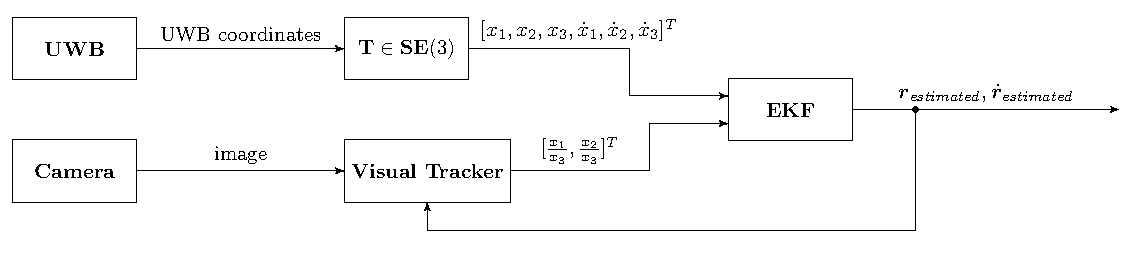
\includegraphics[width=\linewidth]{gfx/blockdiagram_setup}
	
	The states: $\vec x = [\vec r, \dot{\vec{r}}]^T$ with positon $\vec r \in \mathbb{R}^3$, velocity $\dot{\vec r} \in \mathbb{R}^3$\\
	System model:
	\begin{align*}
	\vec x(k) = 
	\begin{bmatrix}
		\textbf{I}_3 & \Delta \textbf{T}\\
		\textbf{0} & \textbf{I}_3
	\end{bmatrix}\vec x(k-1) + \vec v(k-1))\\
	\vec v(k-1) \sim \mathcal{N}(\vec 0, \textbf{Q})
	\end{align*}
}

\note {
	Measurements:\\
	\begin{itemize}
	\item A direct measurement of the state $\vec x$ from UWB multilateration:
	\begin{align*}
	\vec z_1(k) = \textbf{I}_6 \vec x(k) + \vec w_1(k)\\
	\vec \omega_1(k) \sim \mathcal{N}(\vec 0, \textbf{R}_1)
	\end{align*}
	\item A projection of the position $\vec r$ as seen by a camera:
	\begin{align*}
	\vec z_2(k) = \begin{bmatrix}
	x_1(k)/x_3(k)\\
	x_2(k)/x_3(k)
	\end{bmatrix} + \vec w_2(k))\\
	\vec \omega_2(k) \sim \mathcal{N}(\vec 0, \textbf{R}_2)
	\end{align*}
	\end{itemize}
}

\frame { \frametitle{Fusing with an Extended Kalman Filter (EKF)}
	\begin{itemize}
	\item Step 1:\\
	Make a prediction for the mean of the states $\hat{\vec x}_p(k)$ and the co-variance matrix $\textbf{P}_p(k)$:
	\item Step 2:\\
	The information gained from the measurements is used to perform an a posteriori update, resulting in a updated mean of the states $\hat{\vec x}_m(k)$ and an updated co-variance matrix $\textbf{P}_m(k)$.
	\end{itemize}
}

\begin{frame}
	\frametitle{Re-detection}
	\section{Re-detection}
	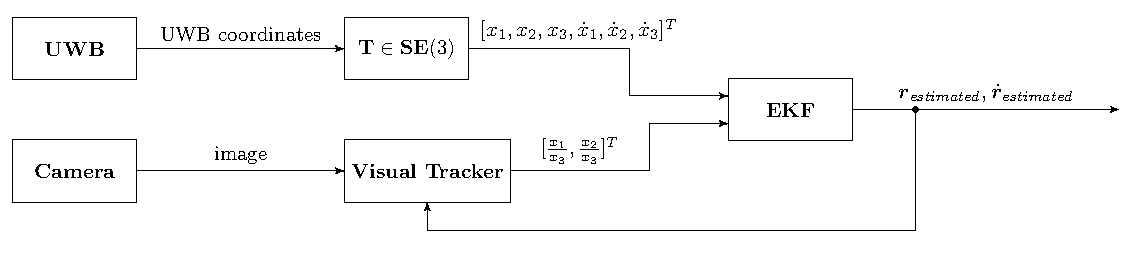
\includegraphics[width=\linewidth]{gfx/blockdiagram_setup}
	\begin{algorithm}[H]
	\tiny
	\begin{algorithmic}[1]
	\While{true}
	\If{target not detected}
	\State Adapt $\textit{PSR}$ and $\textit{response threshold}$
	\State Set re-detection = true
	\Else
	\If{Object was detected in 5 consecutive frames}
	\State Reset $\textit{PSR}$ and $\textit{response threshold}$
	\State Set re-detection flag = false
	\EndIf
	\EndIf
	\If{re-detection flag = true}
	\State Take 2D position from EKF
	\EndIf
	\EndWhile
	\end{algorithmic}
	\end{algorithm}
\end{frame}

\begin{frame}
	\frametitle{Results}
	\section{Results}
	 The $\textit{rmse}$ and the $\textit{rmse}_{xy}$ of the EKF were significantly lower ($> 50\%$) compared with the $\textit{rmse}$ and the $\textit{rmse}_{xy}$ of the UWB system (For the casee, where the visual tracker found the object).\\
	%\tiny
	%\begin{table}
%		\begin{center}
%			\begin{tabular}{c|c|c|c|c}
%				Experiment number & $\textit{rmse}$ of UWB & $\textit{rmse}$ of EKF & $\textit{rmse}_{xy}$ of UWB & $\textit{rmse}_{xy}$ of EKF\\ 
%				\hline 
%				1 & 0.0667 & 0.0350 & 0.0621 & 0.0270 \\
%				2 & 0.0771 & 0.0364 & 0.0734 & 0.0260 \\
%				3 & 0.1304 & 0.0379 & 0.1275 & 0.0312 \\
%				4 & 0.1169 & 0.0344 & 0.1126 & 0.0265 \\
%				5* & 0.1273 & 0.1195 & 0.1159 & 0.1055
				%\hline 
%			\end{tabular}
%		\end{center}
%	\end{table}
%	\normalsize
	\vspace{1cm}
	See demo video!
\end{frame}

\begin{frame}
\frametitle{Results - Demo}
\begin{center}
\href{run:demo_cut_resize.mkv?autostart&start=0}{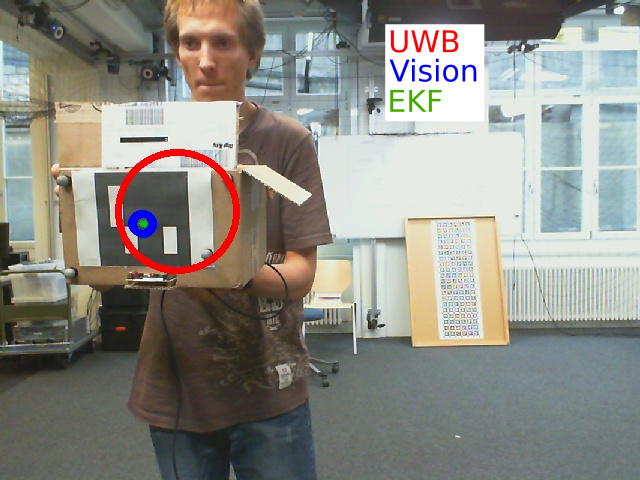
\includegraphics[width=0.9\linewidth]{gfx/2d_output}}
\end{center}
\end{frame}

\frame { \frametitle{Conclusion/Limitation}
	\section{Conclusion}
	\subsection{Conclusion}
	Conclusion:
	\begin{itemize}
	\item The proposed method of fusing UWB and visual tracker impoved the accuracy
	\item The implemented re-detection mechanism performs well
	\end{itemize}

	\subsection{Limitation}
	Limitation:
	\begin{itemize}
	\item The EKF does not consists of an outlier-detection
	\end{itemize}
}

\frame { \frametitle{Outlook}	
	\subsection{Outlook}
	Outlook:
	\begin{itemize}
	\item C++ implementation for usage with higher frequency
	\item More sophisticated re-detection
	\item Calibration of the UWB system with the help of ArUco
	\item Automatic target detection
	\item Multi target tracking
	\end{itemize}
}

\frame { \frametitle{Questions}
	\section{Questions}
	\begin{center}
	
\includegraphics[height=0.75\textheight]{gfx/q&a.jpg}
	\end{center}
}

\frame{ \frametitle{References}
	\section{References}
	\bibliography{graphics}
}

\end{document}